

In this section, risks of the project are obtained from brainstorming. They are analyzed from different angles and among which, critical risks will be assessed further.   
\subsection{Risk Analysis Methodology}
The methodology adopted to conduct the risk analysis is described as following steps:  
\begin{enumerate}[itemsep=0pt, topsep=3pt, partopsep=3pt]
  \item Identify potential risks;
  \item Determine probability;
  \item Determine Impact.
\end{enumerate}

As long as all possible risks are identified after brainstorming, they will be assessed according to the probability and impact respectively. Each aspect has a scale of 1, 3, and 9. A bigger number implies that the risk is more likely to happen or has a more serious consequence. Those risks of interest will be analyzed further based on their risk rating, which is defined as the product of probability and impact. The risk matrix is shown in \ref{fig:riskmatrix}.  


\begin{figure}[h!]
\centering
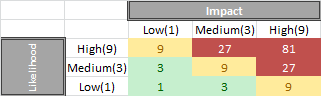
\includegraphics[scale=1.0]{Pictures/riskmatrix.png}
\caption{Risk Matrix : upper right red area implies risks to be offered with action plan; green and yellow area is below tolerance level }
\label{fig:riskmatrix}
\end{figure}

A risk matrix is shown in Table 1. The risks that lies in the upper right in red exceeds the level of tolerance and needs to be made action plan for. 
\subsection{Risk Log}
After the possible risks are identified, they are kept in table 2 following the priority of risk rating. The possible risks with high risk rating are marked in red and will be provided with an action plan below. 

\begin{table}[H]
\caption{Risk Log}
	\label{table:risk}
	\begin{center}
		\begin{tabular}{|c|c|c|c|c|}
			\hline
			\makecell{\textbf{No.}} & \makecell{\textbf{Priority Hazard}} & \makecell{\textbf{Prob.}\\\textbf{(1-9)}} & \makecell{\textbf{Imp.}\\\textbf{(1-9)}} & \makecell{\textbf{Risk Rating}\\\textbf{(Prob.$\times$ Imp.)}} \\ \hline
			\makecell{1} & \makecell{ Estimates are inaccurate} & \makecell{9} & \makecell{9} & \makecell{\textcolor{red}{81}} \\
			\hline
			\makecell{2} & \makecell{ Code error } & \makecell{3} & \makecell{9} & \makecell{\textcolor{red}{27}} \\
			\hline
			\makecell{3} & \makecell{ Failure to follow the methodology } & \makecell{3} & \makecell{9} & \makecell{\textcolor{red}{27}} \\
			\hline
			\makecell{4} & \makecell{ Preparation is inadequate } & \makecell{3} & \makecell{3} & \makecell{9} \\
			\hline
			\makecell{5} & \makecell{ Knowledge integration} & \makecell{3} & \makecell{3} & \makecell{9} \\
			\hline
			\makecell{6} & \makecell{ Info loss during communication} & \makecell{3} & \makecell{3} & \makecell{9} \\
			\hline
			\makecell{7} & \makecell{ Ambiguous goal} & \makecell{1} & \makecell{9} & \makecell{9} \\
			\hline
			\makecell{8} & \makecell{ Disagreement with the coa} & \makecell{1} & \makecell{9} & \makecell{9} \\
			\hline
			\makecell{9} & \makecell{Low morale (interests lost)} & \makecell{1} & \makecell{9} & \makecell{9} \\
			\hline
			\makecell{10} & \makecell{ Tool selection problem} & \makecell{1} & \makecell{3} & \makecell{3} \\
			\hline
			\makecell{11} & \makecell{ Software collapse} & \makecell{1} & \makecell{3} & \makecell{3} \\
			\hline
			\makecell{12} & \makecell{ Misunderstand the requirement} & \makecell{1} & \makecell{3} & \makecell{3} \\
			\hline
		\end{tabular}
	\end{center}
	
\end{table}

\subsection{Action Plan}

An action plan is made for those risks with the highest likelihood and/or consequence. So the risks with risk rating above 9 are provided with the corresponding action plans. The following tables \ref{table:item1}, \ref{table:item2} and \ref{table:item3} provide the action plans of items with high risk ratings.

\begin{table}[h]
\centering
\caption{Action Plan for Item 1}
\label{table:item1}
\begin{tabular}{|l|l|}
\hline
\makecell{\textbf{Risk}}                                                                                                                                                                                  & \makecell{Estimates are inaccurate}                                                                                                                                                                                                                                                                             \\ \hline
\makecell{\textbf{Location/Function}}                                                                                                                                                                     & \makecell{N/A}                                                                                                                                                                                                                                                                                                  \\ \hline
\multicolumn{2}{|c|}{\begin{tabular}[c]{@{}l@{}}\makecell{Summary (RECOMMENDED RESPONSE AND IMPACT)}\end{tabular}}\\ \hline 
\multicolumn{2}{|l|}{\begin{tabular}[c]{@{}l@{}}Inaccurate estimation is a common project risk and especially happens\\ frequently for rookies. This risk will cause a series of project failure and the\\ results of the project almost cannot be achieved. Gaining more\\ experience can be a solution to this problem. \\It is recommended to consult the coach and learning from previous\\ cases when making then estimation.\end{tabular}} \\ \hline
1)Proposed Actions                                                                                                                                                                    & \begin{tabular}[c]{@{}l@{}}Make considerate estimates patiently\\ Check the progress regularly\\ Consult with the coach\end{tabular}                                                                                                                                                                 \\ \hline
2)Resource Requirements                                                                                                                                                               & \begin{tabular}[c]{@{}l@{}}Time of the coach\\ Previous similar project case\\ Planned schedule\end{tabular}                                                                                                                                                                                         \\ \hline
3)Responsibilities                                                                                                                                                                    & \begin{tabular}[c]{@{}l@{}}The coach to be consulted about\\ estimation rationality                                                                                                                                                                                                                                             
\end{tabular}                                                                                                                                                                                         \\ \hline
4)Timing                                                                                                                                                                              & \begin{tabular}[c]{@{}l@{}}Present the estimation at the nearest meeting\\ after it is made.\\Check the progress once a week\end{tabular}                                                                                                                                                              \\ \hline
5)Reporting/Monitoring                                                                                                                                                                & \begin{tabular}[c]{@{}l@{}}Each member has a milestone or individual sched-\\-ule to achieve within given time\end{tabular}                                                                                                                                                                           \\ \hline
\end{tabular}
\end{table}

\begin{table}[h]
\centering
\caption{Action Plan for Item 2}
\label{table:item2}
\begin{tabular}{|l|l|}
\hline
\makecell{\textbf{Risk}}                                                                                                              & \makecell{Code errors}                                                                                                                                                                                                                        \\ \hline
\makecell{\textbf{Location/Function}}                                                                                                 & \makecell{Solver}                                                                                                                                                                                                                             \\ \hline
\multicolumn{2}{|c|}{\begin{tabular}[c]{@{}l@{}}\makecell{Summary (RECOMMENDED RESPONSE AND IMPACT)}\end{tabular}} \\ \hline
\multicolumn{2}{|l|}{\begin{tabular}[c]{@{}l@{}}Handling the code errorscan be time-consuming. To ensure that the program-\\mer  familiar with the expected results and reflect the idea to the code accur-\\ately.\end{tabular}} \\ \hline
1)Proposed Actions                                                                                                & \begin{tabular}[c]{@{}l@{}}Test the code by comparing the results with the\\ expected ones\\ Read through the code logically\end{tabular}                                                                                          \\ \hline
2)Resource Requirements                                                                                           & \begin{tabular}[c]{@{}l@{}}Time of the programmer\\ Computer with installed related software\\ Data from the previous work\end{tabular}                                                                                            \\ \hline
3)Responsibilities                                                                                                & Programmer within the group                                                                                                                                                                                                        \\ \hline
4)Timing                                                                                                          & \begin{tabular}[c]{@{}l@{}}Check the code segments while coding\\ Test the code after finishing coding\end{tabular}                                                                                                                \\ \hline
5)Reporting/Monitoring                                                                                            & \begin{tabular}[c]{@{}l@{}}Data documentation of previous work\\ The report of new data to be finished\end{tabular}                                                                                                                \\ \hline
\end{tabular}

\end{table}

\begin{table}[h]
\centering
\caption{Action Plan for Item 3}
\label{table:item3}
\begin{tabular}{|l|l|}
\hline
\makecell{\textbf{Risk}}                                              & \makecell{Failure to follow the methodology}                                                                                                                                                                       \\ \hline
\makecell{\textbf{Location/Function}}                                 & \makecell{Methodology }                                                                                                                                                                                            \\ \hline
\multicolumn{2}{|c|}{\begin{tabular}[c]{@{}l@{}}\makecell{Summary (RECOMMENDED RESPONSE AND IMPACT)}\end{tabular}}\\ \hline 
\multicolumn{2}{|l|}{\begin{tabular}[c]{@{}l@{}}To ensure that each member get the individual work done within the deadline \\ To ensure that the work is formulated based on the methodology.\end{tabular}} \\ \hline
1)Proposed Actions                                & \begin{tabular}[c]{@{}l@{}}Set reasonable milestones and regular deadlines\\ Check the achievement according to the schedule\\ Formulate the work by methodology\end{tabular}                           \\ \hline
2)Resource Requirements                           & Methodology to be adopted                                                                                                                                                                               \\ \hline
3)Responsibilities                                & Everyone                                                                                                                                                                                                \\ \hline
4)Timing                                          & \begin{tabular}[c]{@{}l@{}}Get the work done before the deadline\\ Set milestones after work formulation\end{tabular}                                                                                   \\ \hline
5)Reporting/Monitoring                            & \begin{tabular}[c]{@{}l@{}}Schedule or milestone plan report\end{tabular}                                                                                                                             \\ \hline
\end{tabular}
\end{table}
\FloatBarrier

